

\chapter{Experiments and Results} \label{ch:experiments_and_results}
To analyze the SCOUt control schema, three instances of a SCOUt controller are trained and then tested in two experiments.
The first experiment compares the performance of each

\noindent
SCOUt controller against a random and heuristic controller to determine if they exhibit intelligent behavior when attempting to complete a given goal.
The second experiment tests adaptability of the controllers by removing sensors or changing the goal and providing additional training for new goals.
This will create new situations for which the controllers have not been trained.
Two different goals are used in these experiments: \textit{Find Human} and \textit{Map Water}.
\textit{Find Human} requires the agent to search an environment to locate a \texttt{Human} anomaly randomly placed within the environment.
\texttt{Human} is an extended class of the \texttt{Anomaly} trait, and its definition can be found in Appendix~A-7.
Goal completion is either 100 percent for successfully locating the human, or 0 percent for failing to find the human before health or energy has been depleted.
For the goal to be successfully completed, the controller must navigate to one of the eight cells adjacent to the Human anomaly's location in the environment (figure~\ref{fig:human_discovery_zone}).
\textit{Map Water} tests a controller's ability to navigate within an environment and collect as much water depth data as possible.
\textit{Map Water} operations will run until the entire area has been scanned for water depth, or the agent has depleted its health or energy.
Goal completion is then reward based on the percentage of the environment that was scanned for water depth.
Training and testing are both conducted using three different \texttt{EnvironmentTemplates}.
Templates differs in their difficulty to navigate due to the modifications present within them.
For example, more difficult templates will generate larger environments to explore that contain more hazardous terrain modifications.

\begin{figure}[!htb]
  \centering
  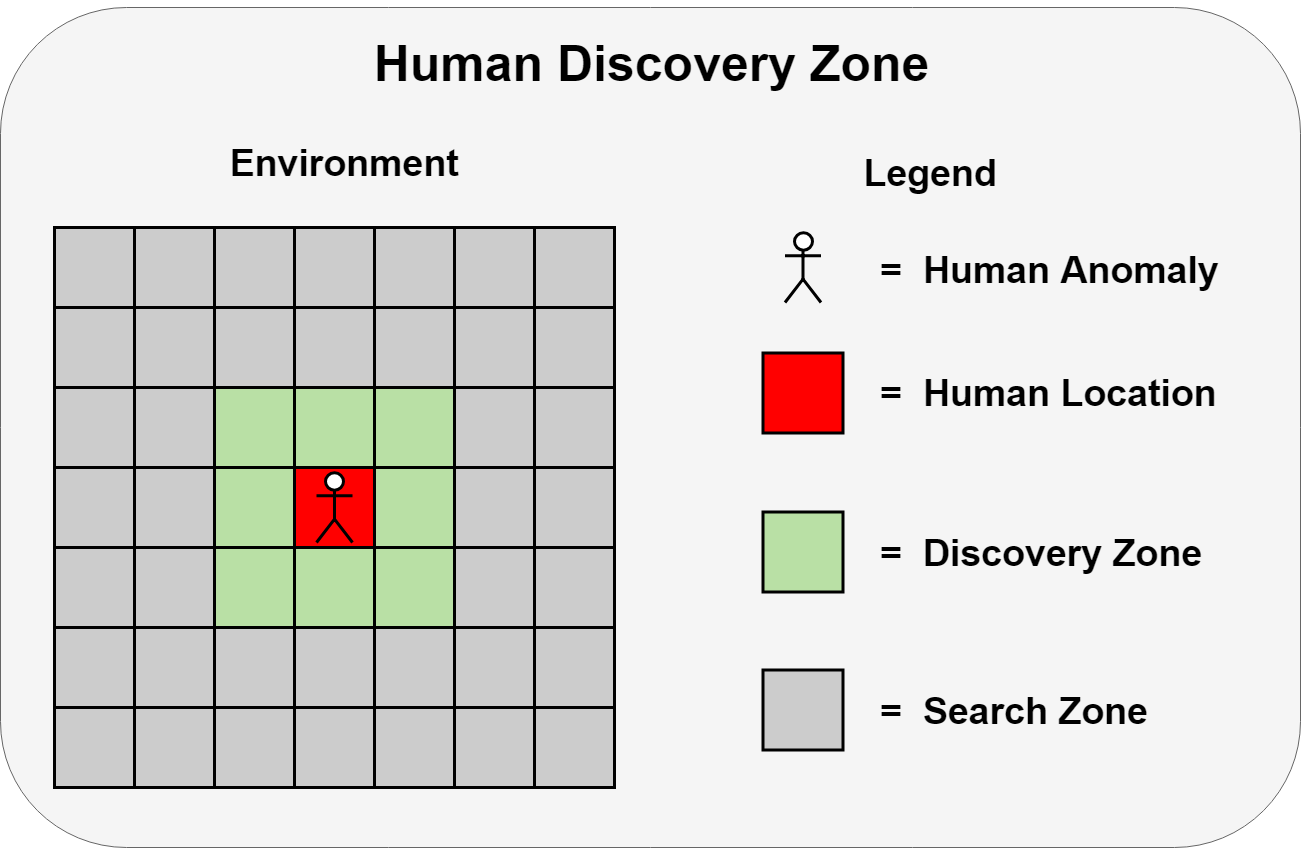
\includegraphics[width=0.8\columnwidth]{Figures/human_discovery_zone.png}
  \caption[Human Discovery Area]{Diagram of the area in an environment that an agent must navigate to in order to ``discover'' a human anomaly. This applies to operations where the goal is \textit{Find Human}.}
  \label{fig:human_discovery_zone}
\end{figure}

% \todo{testing fig}

During both training and experimentation, tests are conducted to measure the performance of each controller.
A test is a series of operations that an agent will attempt to complete using a given set of sensors.
Each operation in the series will be run once per controller, where each run is identical: same goal, same environment instance, same starting position, and same agent setup (aside from the controller that is used).
The only exception to this is in Experiment 2 (section~\ref{sec:experiment2}), when sensors are removed from the SCOUt controller's agent to test adaptability.
Tests will measure the performance of several controllers in these identical operations to see how they compare.
Each test will include at least one random, one heuristic and one SCOUt controller.
Two different heuristic controllers are used in testing depending on the goal of the operation.
$Heuristic_{FH}$ and $Heuristic_{MW}$ are used for \textit{Find Human} and \textit{Map Water} operations, respectively.
The random and heuristic controllers provide baselines for performance of the SCOUt controllers.
These baselines are important as the difficulty of an operation is difficult to predict.
Different instances of the same operation setup can yield unique environments and starting positions that will alter the difficulty of goal completion, or even prevent it entirely.
Performance is measured in four categories: goal completion, the number of actions taken, remaining health and remaining energy.
Additionally, the agent's starting location for each operation will be chosen in a location that does not result in damage (e.g., starting in a cell with water present) or immediate goal completion (e.g., starting next to the Human anomaly).
The specific agent setups and \texttt{EnvironmentTemplates} used for training and experimentation are covered in sections~\ref{sec:agent_setups} and~\ref{sec:test_environment_templates}.


\section{Agent Setup} \label{sec:agent_setups}
% \todo{diagram}
A similar agent setup is used for every operation in training and testing.
The only variation is in the controller being used and the sensor types present.
All health, energy, mobility and durability variables will be set to the same value throughout training and experimentation.
This will ensure that no advantage or disadvantage is given to any controller when navigating the agent through an environment.
The performance of each controller will then solely be reflected by their usage of available sensors, and analyses of the data they collect.
Different sensors are available for use depending on the goal, or in the unique case where the set of equipped sensors are changed tests in Experiment 1 (section~\ref{sec:sensor_change}), depending on the test setup.
Four sensors are used throughout testing: elevation, temperature, decibel and water.
When sensors are available for an agent to use, the indicator flag will reflect their usage for the present goal.
For \textit{Find Human} the temperature and decibel sensors will be flagged as indicators, and for \textit{Map Water} the water sensor will be flagged as an indicator.
Water and elevation sensors are always flagged as hazard since the defined agent \texttt{Durability} and \texttt{Mobility} instances make the agent susceptible to water and fall damage.
Each agent will always begin an operation with an empty \texttt{internalMap}, 100.0 \texttt{health} and a starting \texttt{energyLevel} of 100.0.
The instances of the \texttt{Agent}, \texttt{Mobility}, \texttt{Durabilities}, and each \texttt{Sensor} used in training and testing are found in Appendix~E-1.


\section{Environment Templates} \label{sec:test_environment_templates}
Three \texttt{EnvironmentTemplate}s with increasing difficulty are created for use in training and experimentation (\textit{EASY}, \textit{MEDIUM}, and \textit{HARD}).
Change in difficulty is achieved by adjusting: environment size, presence of \texttt{TerrainModification}s, average and deviation values of each \texttt{ElementSeed}, and the values within each \texttt{Effect} of any \texttt{Anomaly} present.
Increased environment size creates a wider area that an agent will have to explore.
More

\noindent
\texttt{TerrainModification}s makes each environment potentially more hazardous.
Hills and valleys can create areas with the potential of fall damage or the inability to climb slopes, and pools and streams of water will create areas that will damage an agent that enters them.
Changing the average and deviation values of \texttt{ElementSeed}s used to generate the \texttt{Environment} instance has a couple of effects.
As an example, by increasing the average decibel values in the environment, the distinction of the human's decibel \texttt{Effect} is dampened, and the agent will need to navigate closer to the source in order to detect any noise produced.
Also, if the variance in decibel values increases, it becomes more difficult for an agent to distinguish what levels of increase are considered significant enough to investigate.
Last, by adjusting the values within \texttt{Anomaly} \texttt{Effect}s, it can become harder for an intelligent controller to detect the \texttt{Anomaly} from a distance.
For example, by reducing the decibel effect of a \texttt{Human Anomaly}, the radiation of the effect will cover less area in the environment, meaning the agent will have to search longer before it may pick up on the effect.

Each environment template has one \texttt{Human} that will be placed into it at random in a non-hazardous zone.
The same templates will then be used for both the \textit{Find Human} and \textit{Map Water} goals.
In the case that the goal is \textit{Map Water}, a \texttt{Human Anomaly} will still be present within the environment, but it can be ignored by the agent.
Each of these \texttt{EnvironmentTemplate}s are listed in JSON format in Appendix~E-2, Appendix~E-3, and Appendix~E-4.
When a template is used in training or experimentation, it will be loaded from its file, converted to a Scala object, and passed to the \texttt{EnvironmentBuilder}.
The resulting \texttt{Environment} instance can then be used in one or more test operations.


\section{Training} \label{sec:training}
Three separate SCOUt controllers are trained to accumulate memory pools of state-action rewards.
Each of the three controllers are trained with different goal configurations but follow the same training process (figure~\ref{fig:training_diagram}).
One is trained using the \textit{Find Human} goal, the second using the \textit{Map Water} goal and the third is a hybrid, trained using both goals.
They are named $SCOUt_{FH}$, $SCOUt_{MW}$ and $SCOUt_{H}$ respectively.
Each controller is trained for 30 iterations, where an iteration runs one operation per environment template.
Once training has completed, each controller will have collected state-action rewards (SAR) from a total of 90 operations (30 on EASY, 30 on MEDIUM and 30 on HARD).
Every operation that $SCOUt_{FH}$ is run in will be with the \textit{Find Human} goal and every operation for $SCOUt_{MW}$ will be with the \textit{Map Water} goal.
$SCOUt_{H}$ will alternate goals for each iteration.
In total it will have run 45 operations with the \textit{Find Human} goal and 45 operations with the \textit{Map Water} goal (15 on EASY, 15 on MEDIUM and 15 on HARD for each).

\begin{figure}[H]
  \centering
  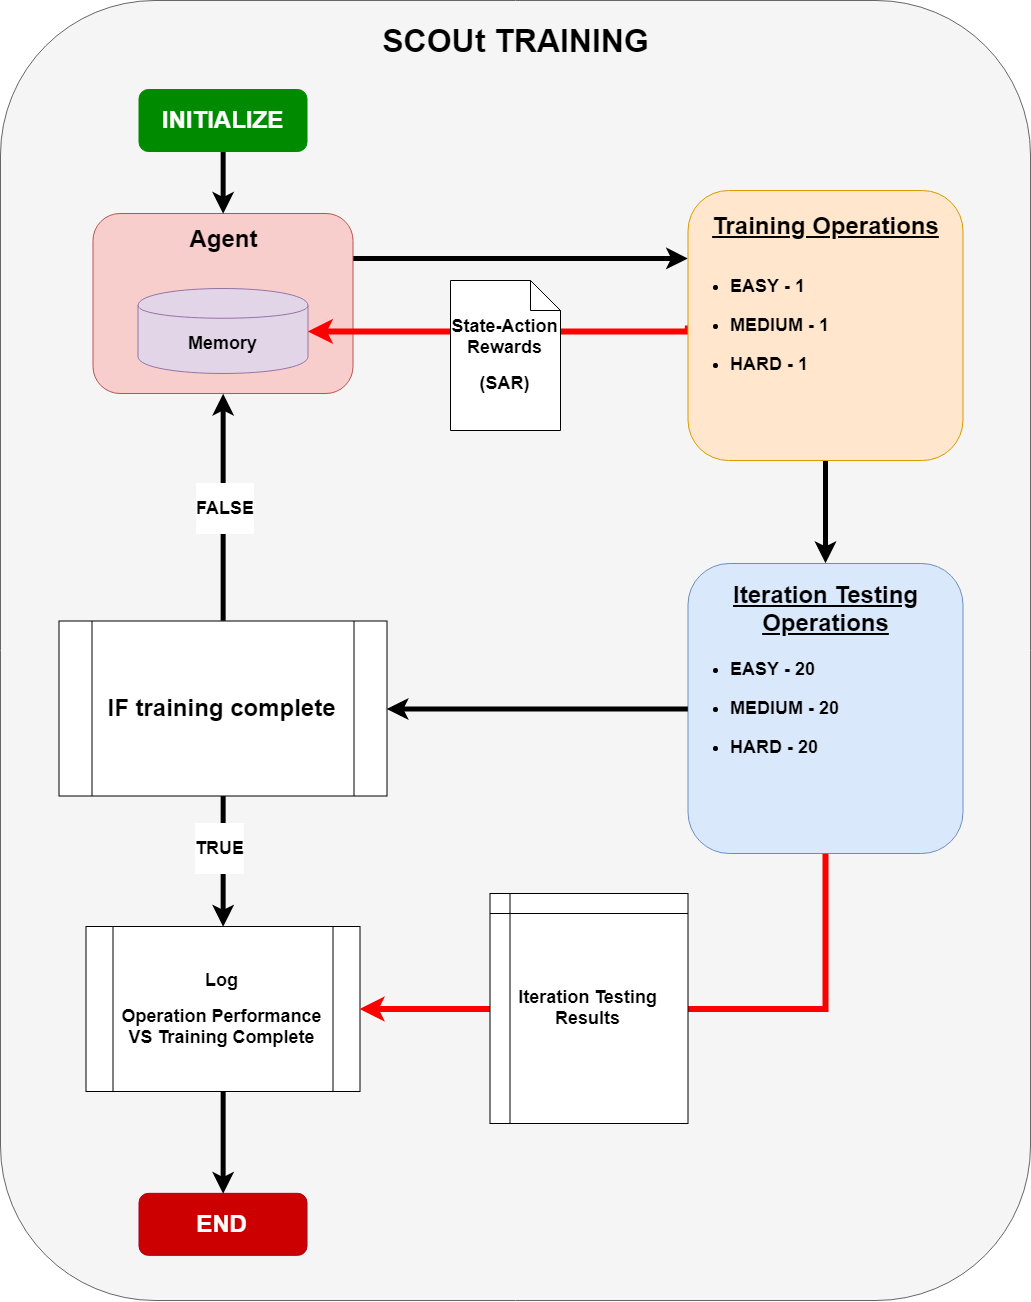
\includegraphics[width=0.7\columnwidth]{Figures/training_diagram.png}
  \caption[SCOUt Memory Training Process]{This diagram shows the training process that each SCOUt controller will follow. Training is completed after 30 iterations of the process. The number of operations for each environment difficulty in training and in iteration testing are shown. The goal for the operation will depend on the specific SCOUt controller that is being trained.}
  \label{fig:training_diagram}
\end{figure}

After each training iteration, the controller is tested with its current memory to track performance improvements.
Testing at each iteration runs a series of simulated operations to collect performance data.
Each series uses the controller's respective goal(s) and is run on each testing environment template 20 times (20 on EASY, 20 on MEDIUM, and 20 on HARD).
The controller tested will have access to its current memory pool that it has gathered during all of the training operations it has completed so far.
As the purpose of iteration testing is to measure the \textit{current} performance level of the controller, no SARs will be gathered during these tests and the memory will be left un-altered.
For a baseline, the $Random$ controller is run through the same series of tests.
Results from the 60 total operations will be averaged in each of the four performance categories.
The averaged results of the learning SCOUt controller will then be differenced against the averaged results of the $Random$ controller.
By differencing the averages, it can be observed how much better or worse the SCOUt controller was able to perform than the $Random$ controller in the same testing conditions.
This also removes the discrepancy between each iteration test that is run, as one iteration text may have generated a series of exceptionally difficult or easy operations.
It is expected that as training continues, the goal completion, remaining health and remaining energy performances of SCOUt will increase, and the number of actions performed will decrease when compared against the $Random$ controller.

\subsection{Initial Training Results}
Results for $SCOUt_{FH}$ training (figure~\ref{fig:findhuman_training_results}) show the desired trends of increased performance over training iterations.
Average goal completion and average remaining energy begin at the same performance levels as $Random$ and increase to be consistently better than random over time.
The average number of actions performed begins slightly below $Random$ and continue to decrease before leveling out roughly two-thirds of the way through training.
This demonstrates that the controller is learning to perform more efficiently over time, as both average goal completion and average remaining health show major performance boosts, while fewer actions are being used.
The average remaining health of $SCOUt_{FH}$ shows slight increase over training, but for the most part is equivalent to that of the $Random$ controller.

% \todo{Improve captions}
\begin{figure}[H]
  \centering
  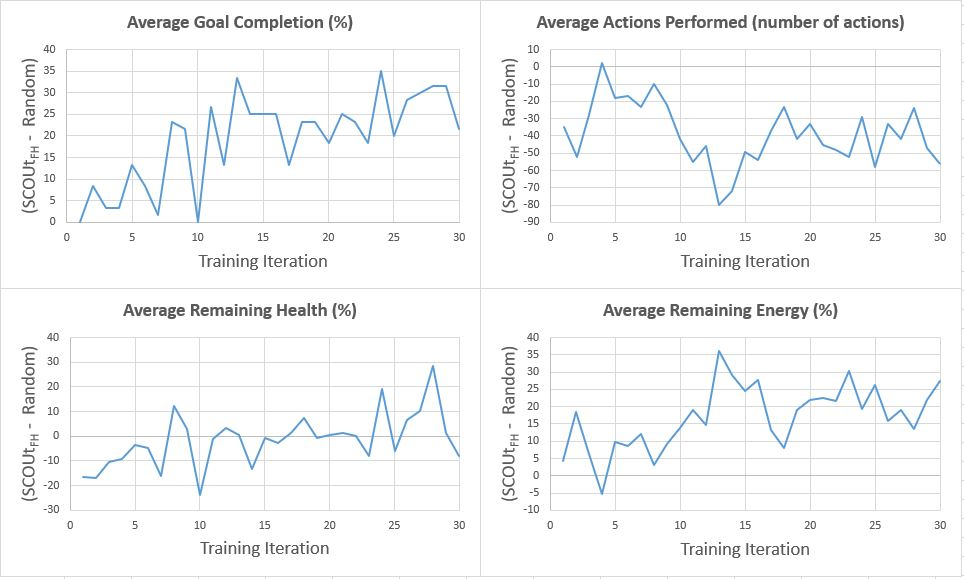
\includegraphics[width=1.0\columnwidth]{Figures/Results/Training/SCOUt-FindHuman.JPG}
  \caption[Iteration Testing Performance Results: $SCOUt_{FH}$]{Iteration testing performance results for $SCOUt_{FH}$ attempting \textit{Find Human}. All graphs show the controller's average difference in performance compared to $Random$ ($SCOUt_{FH}$ average - $Random$ average) VS the number of training iterations completed.}
  \label{fig:findhuman_training_results}
\end{figure}

Results for $SCOUt_{MW}$ (figure~\ref{fig:mapwater_training_results}) are less positive.
Average goal completion and average remaining health both decrease during the first half of training but begin to show upward trends toward the end.
While the average goal completion of $SCOUt_{MW}$ is consistently better than $Random$'s, the average remaining health actually performs worse throughout iteration testing.
$SCOUt_{MW}$ does perform well in the average number of actions taken per operation, however this is likely due to the fact that health is depleted (agent navigating into water) and the operation is ended early.
The same can be said for the remaining energy, as there will be a larger amount of energy remaining after an operation is ended due to depletion of health.
The reason for these poor performance results seem to be tied with the agent's inability to avoid hazardous areas containing water.
Training was repeated using different setups to see if results could be improved.
These repeated training runs are discussed in subsection~\ref{subsec:training_variations}.
Despite unimpressive training results, $SCOUt_{MW}$ still performs well in the tests to follow.

\begin{figure}[H]
  \centering
  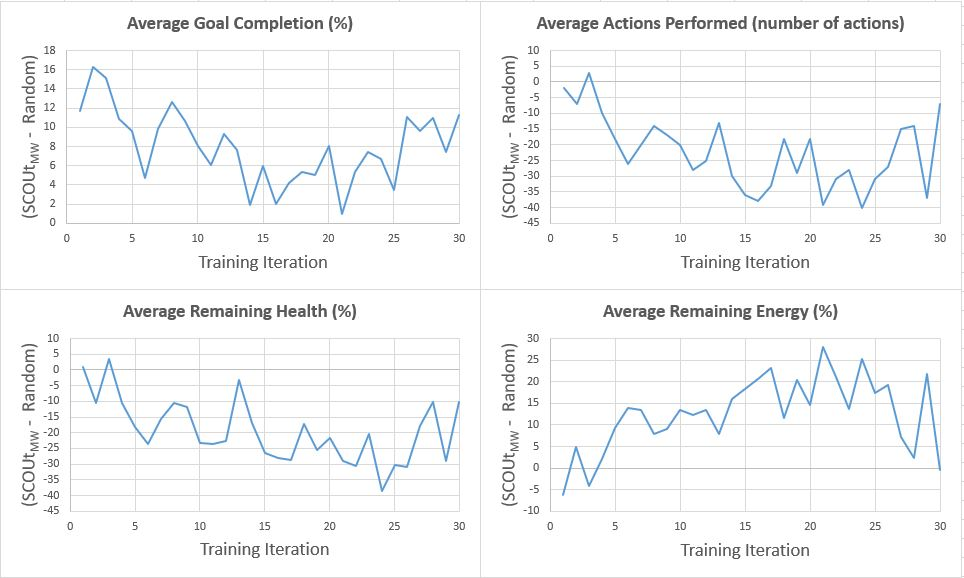
\includegraphics[width=1.0\columnwidth]{Figures/Results/Training/SCOUt-MapWater.JPG}
  \caption[Iteration Testing Performance Results: $SCOUt_{MW}$]{Iteration testing performance results for $SCOUt_{MW}$ attempting \textit{Map Water}. All graphs show the controller's average difference in performance compared to $Random$ ($SCOUt_{MW}$ average - $Random$ average) VS the number of training iterations completed.}
  \label{fig:mapwater_training_results}
\end{figure}

For $SCOUt_{H}$, performance was tracked for both of the \textit{Find Human} and \textit{Map Water} goals.
The iteration test results over training for each of these are found in figure~\ref{fig:hybrid_training_results_fh} and figure~\ref{fig:hybrid_training_results_mw}.
For the majority of the results in both goal types, the average performance of $SCOUt_{H}$ does not show any major increasing trends.
In \textit{Find Human} testing, average goal completion rises and falls throughout training.
The cause of this is unclear but is likely a side effect of simultaneous training on two goals at once.
We also see a slight upward trend in the average number of actions that are being performed, but it does stay under $Random$'s performance throughout.
Towards the end of training, performances in \textit{Map Water} begin to shift in three categories.
Remaining health and number of actions performed shift up, while remaining energy drops, and average goal completion remains fairly consistent.
While more actions are being taken (resulting in the decrease of remaining energy), it appears that $SCOUt_{H}$ is learning better hazard avoidance behaviors as remaining health has increased over time.
$SCOUt_{H}$ training was also repeated to see if results could be improved (covered in subsection~\ref{subsec:training_variations}).


\begin{figure}[H]
  \centering
  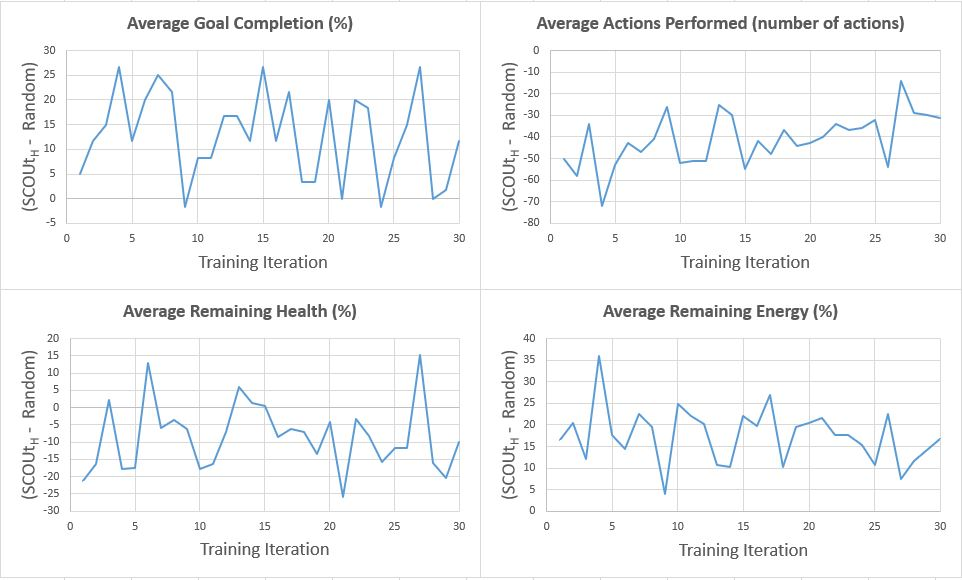
\includegraphics[width=1.0\columnwidth]{Figures/Results/Training/SCOUt-Hybrid-FindHuman.JPG}
  \caption[Iteration Testing Performance Results: $SCOUt_{H}$ (Find Human)]{Iteration testing performance results for $SCOUt_{H}$ attempting \textit{Find Human}. All graphs show the controller's average difference in performance compared to $Random$ ($SCOUt_{H}$ average - $Random$ average) VS the number of training iterations completed.}
  \label{fig:hybrid_training_results_fh}
\end{figure}

\begin{figure}[H]
  \centering
  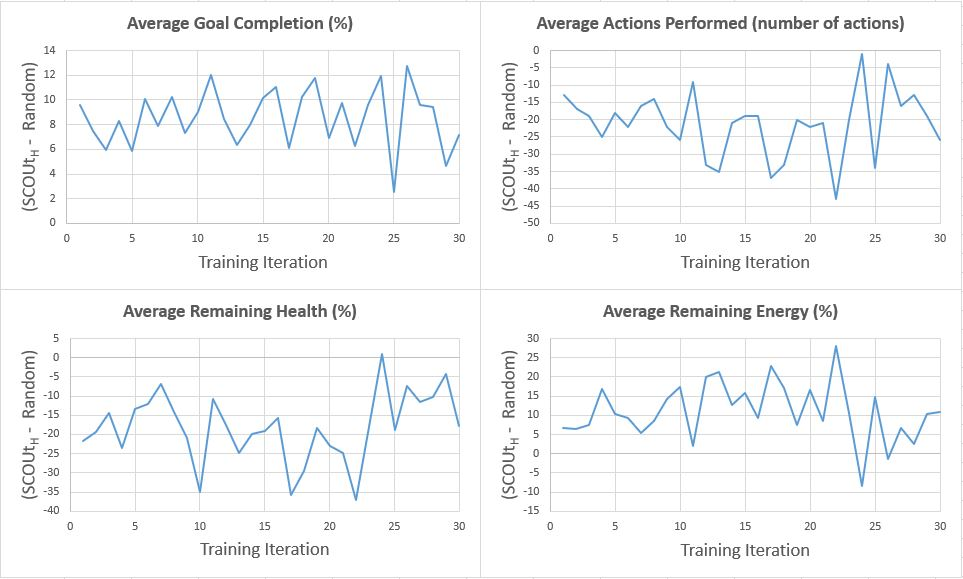
\includegraphics[width=1.0\columnwidth]{Figures/Results/Training/SCOUt-Hybrid-MapWater.JPG}
  \caption[Iteration Testing Performance Results: $SCOUt_{H}$ (Map Water)]{Iteration testing performance results for $SCOUt_{H}$ attempting \textit{Map Water}. All graphs show the controller's average difference in performance compared to $Random$ ($SCOUt_{H}$ average - $Random$ average) VS the number of training iterations completed.}
  \label{fig:hybrid_training_results_mw}
\end{figure}


\subsection{Training Variations} \label{subsec:training_variations}
Two variations of SCOUt controller training were conducted to see if better iteration testing results could be achieved for $SCOUt_{MW}$ and $SCOUt_{H}$.
While $SCOUt_{FH}$ performed well in training, this controller was also retrained using the same variations to assure that there would not be any negative effects to its performance.
The repeated runs altered the way that long-term rewards were calculated at the end of operations, but the same training and iteration testing setup was used: 30 iterations, 1 test on each environment per iteration, 60 operations per iteration test, and iteration testing performance was compared relative to the $Random$ controller.
Variation 1 changed the way that operations factored goal completion into the long-term reward (algorithm~\ref{algorithmic:long_term_reward}).
Instead of always rewarding the controller based on their percent of completion, it would only reward them if the agent had remaining health.
This essentially factors the goal completion as 0 percent if the agent had completely depleted its health.
Effects of this alteration are not expected to cause changes in \textit{Find Human} operations (goal completion is already always 0 unless the human was found), but it should lower the rewards seen in \textit{Map Water} operations since there is typically a portion of the goal completed regardless of how the operation ended.
This variation was made in hope that controllers would learn stronger hazard avoidance behaviors through the harsher long-term reward system.
Variation 2 used the original goal completion equation, but altered the weight used for it.
Instead of \texttt{goalRewardWeight} being set to 1, it was bumped up to 1.5.
This variation was conducted to see if more emphasis was needed on the controllers' level of goal completion within the long-term reward.
If a controller obtained a higher level of goal completion, it must have been able to survive in its environment long enough to do so, which would hopefully counteract the hazard avoidance issue.
Results for all three controllers' in the new training variations are displayed as follows: $SCOUt_{FH}$ - figure~\ref{fig:findhuman_training_comparisons}, $SCOUt_{MW}$ - figure~\ref{fig:mapwater_training_comparisons}, $SCOUt_{H}$ - figures~\ref{fig:hybrid_training_fh_comparisons} and~\ref{fig:hybrid_training_mw_comparisons}.
These graphs show an overlay of the performance results for variation 1, variation 2 and the original training setups that were conducted to easily compare differences between them.
All of the results for variations 1 and 2 can be viewed independently in Appendix~F and Appendix~G.

\begin{figure}[H]
  \centering
  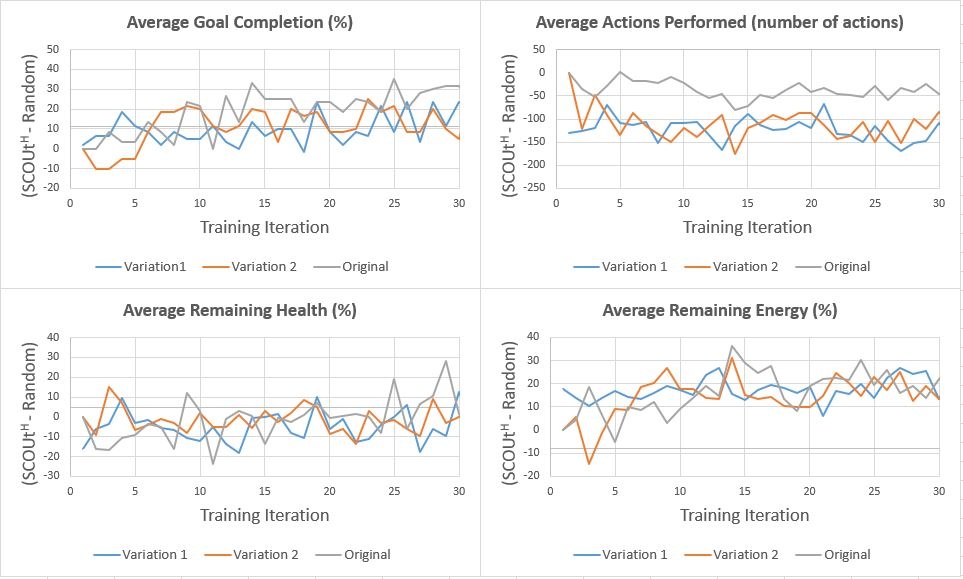
\includegraphics[width=1.0\columnwidth]{Figures/Results/TrainingVariations/FindHuman.JPG}
  \caption[Training Variation Comparisons $SCOUt_{FH}$]{Iteration testing performance results for $SCOUt_{FH}$ attempting \textit{Find Human}. All graphs show the controller's average difference in performance compared to $Random$ ($SCOUt_{FH}$ average - $Random$ average) VS the number of training iterations completed. This graph overlays the results from three different training setups: variation 1, variation 2, and original.}
  \label{fig:findhuman_training_comparisons}
\end{figure}

\begin{figure}[H]
  \centering
  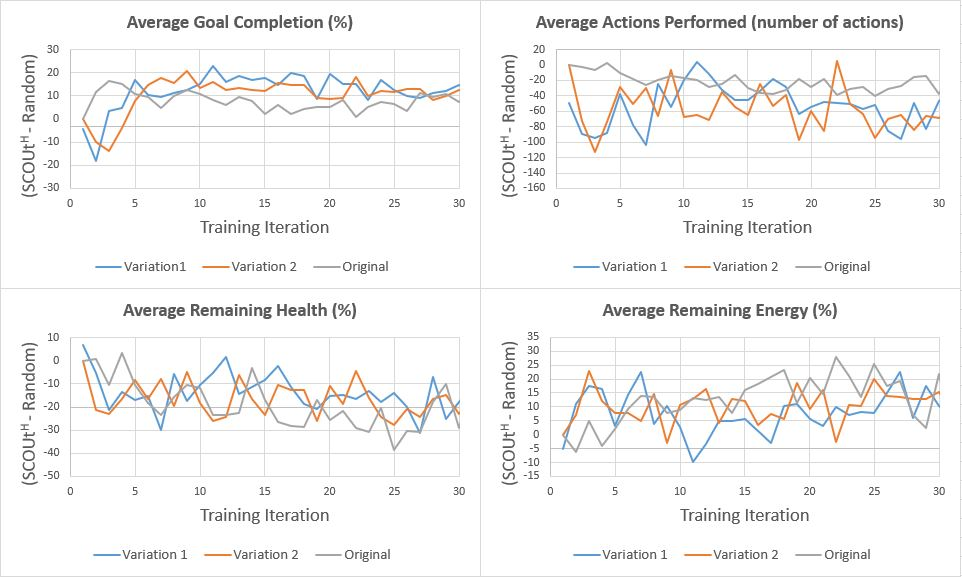
\includegraphics[width=1.0\columnwidth]{Figures/Results/TrainingVariations/MapWater.JPG}
  \caption[Training Variation Comparisons $SCOUt_{MW}$]{Iteration testing performance results for $SCOUt_{MW}$ attempting \textit{Map Water}. All graphs show the controller's average difference in performance compared to $Random$ ($SCOUt_{MW}$ average - $Random$ average) VS the number of training iterations completed. This graph overlays the results from three different training setups: variation 1, variation 2, and original.}
  \label{fig:mapwater_training_comparisons}
\end{figure}

\begin{figure}[H]
  \centering
  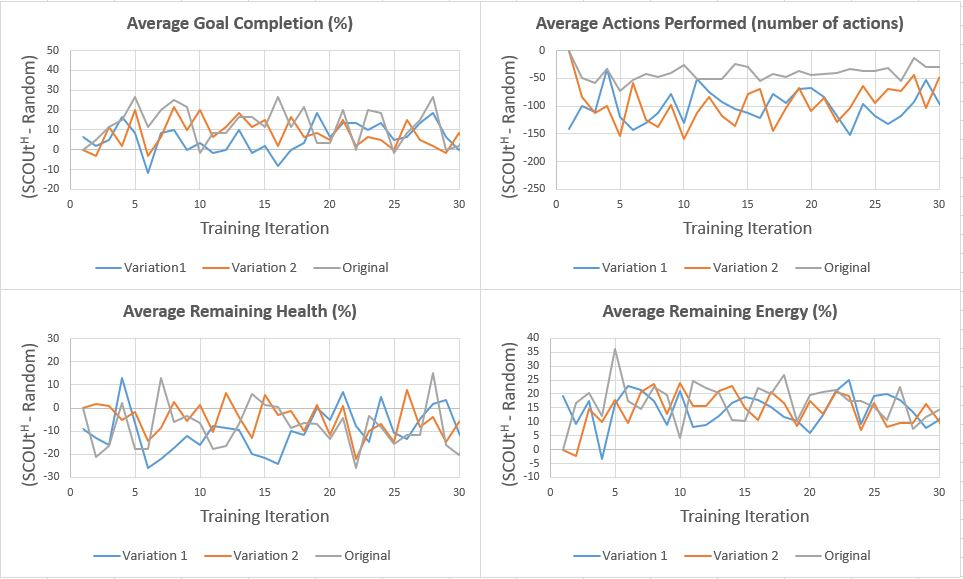
\includegraphics[width=1.0\columnwidth]{Figures/Results/TrainingVariations/Hybrid-FindHuman.JPG}
  \caption[Training Variation Comparisons $SCOUt_{H}$ (Find Human)]{Iteration testing performance results for $SCOUt_{H}$ attempting \textit{FindHuman}. All graphs show the controller's average difference in performance compared to $Random$ ($SCOUt_{H}$ average - $Random$ average) VS the number of training iterations completed. This graph overlays the results from three different training setups: variation 1, variation 2, and original.}
  \label{fig:hybrid_training_fh_comparisons}
\end{figure}

\begin{figure}[H]
  \centering
  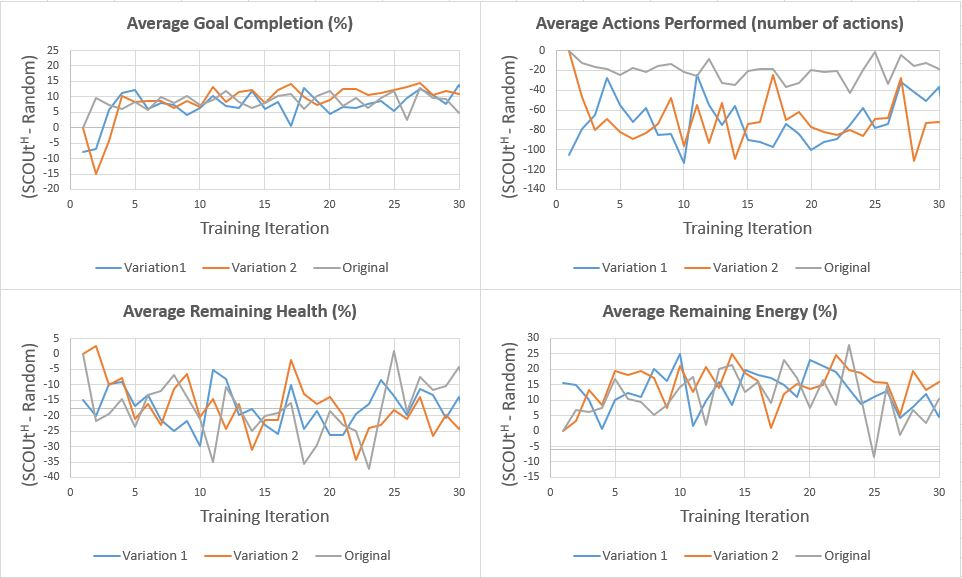
\includegraphics[width=1.0\columnwidth]{Figures/Results/TrainingVariations/Hybrid-MapWater.JPG}
  \caption[Training Variation Comparisons $SCOUt_{H}$ (Map Water)]{Iteration testing performance results for $SCOUt_{H}$ attempting \textit{Map Water}. All graphs show the controller's average difference in performance compared to $Random$ ($SCOUt_{H}$ average - $Random$ average) VS the number of training iterations completed. This graph overlays the results from three different training setups: variation 1, variation 2, and original.}
  \label{fig:hybrid_training_mw_comparisons}
\end{figure}


Performance results show that all of the iteration tests held the same trend lines between each variation of training setup.
Looking at the actual values within each graph, we do see that both variation 1 and 2 hold slightly better results, especially in the category of average actions being performed.
Difference between these two is negligible, so variation 2 was chosen as the winner since it achieved performance boosts through simply adjusting the weighting of goal calculation rather than altering the equation's logic.
For this reason, the following experiments sets the \texttt{goalRewardWeight} to $1.5$ in the long-term reward equation and used the resulting trained memory sets from variation 2 for the SCOUt controllers.



\section{Experiment 1} \label{sec:experiment1}
Once training was completed, the resulting SCOUt controllers were individually tested against $Random$ and their respective heuristic controller.
Tests in Experiment 1 ran a series of 1000 operations per environment template.
The environment template is used to generate 200 unique environments, each of which is used for 5 operations.
Results are averaged for each controller's performance within each of the environment difficulties they were tested in.
It is expected that the SCOUt controllers perform better than $Random$ and as good or better than the heuristic controllers.
This would be reflected in higher average goal completion, average remaining health and average remaining energy, and lower average actions performed.

Results for $SCOUt_{FH}$ (figure~\ref{fig:findhuman_test_results}) show clear superiority across almost every test.
The only area where scout under-performed was in average remaining health.
In the medium difficulty environments, $SCOUt_{FH}$ came in second in this category (right behind $Heuristic_{FH}$) but all three controllers performed within the same 5 percent range.
In the hard difficulty environments, $SCOUt_{FH}$ came in last out of the three in remaining health, but only by a margin of 2 percent.
Average goal completion in every environment difficulty was about double the performance of $Heuristic_{FH}$ and triple the performance of $Random$.
$SCOUt_{FH}$ also outperformed $Heuristic_{FH}$ and $Random$ in both average actions taken and average remaining health.
We see in these results that the heuristic controller was able to perform better than $Random$ in most tests.
The margin of performance difference between $Heuristic_{FH}$ and $Random$ tends to shrink as the environment difficulty is increased.
While goal completion consistently remained above that of $Random$, we can see that $Heuristic_{FH}$ is having to use more actions to achieve the goal.

\begin{figure}[H]
  \centering
  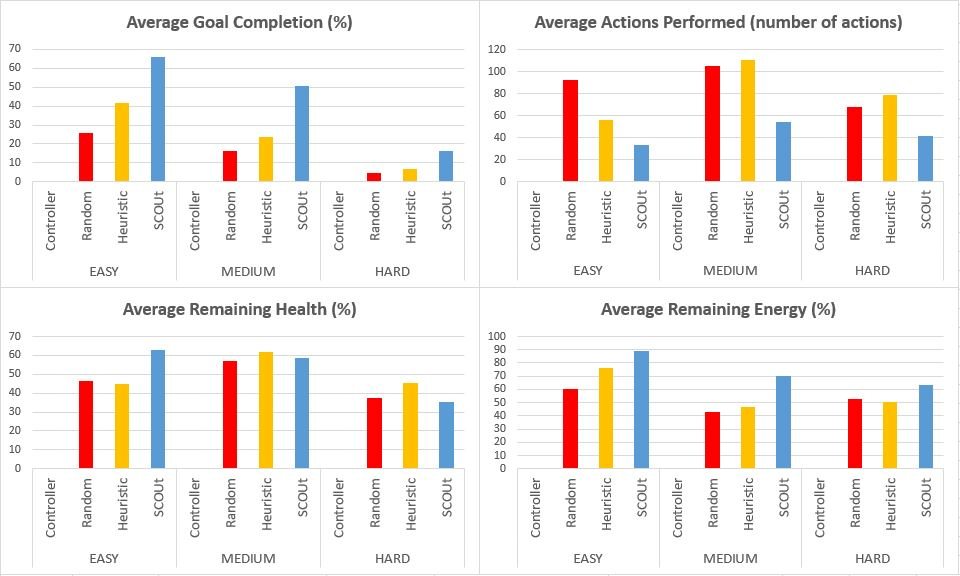
\includegraphics[width=1.0\columnwidth]{Figures/Results/Experiment1/FindHuman.JPG}
  \caption[Experiment 1 Results: $SCOUt_{FH}$]{Performance results for $Random$, $Heuristic_{FH}$ and $SCOUt_{FH}$ controllers attempting \textit{Find Human} in various environment difficulties.}
  \label{fig:findhuman_test_results}
\end{figure}


$SCOUt_{MW}$'s results (figure~\ref{fig:mapwater_test_results}) show performance levels that are mostly superior to $Heuristic_{MW}$ and $Random$, but it does not exhibit the same level of superiority as seen in

\noindent
$SCOUt_{FH}$'s results.
Again, the area where the SCOUt controller is lacking in performance is the average remaining health.
In the easy difficulty environment, $SCOUt_{MW}$ suffers tremendously with an average remaining health of ~9 percent.
Interestingly, the average remaining health increases as environment difficulty increases.
Reasons behind this behavior are unclear as other performance trends increase and decrease as expected when the environment difficulty changes.
$Heuristic_{MW}$ ranks as expected.
The performance values are consistently better than $Random$ in every category outside of average remaining energy.
In this category, $Heuristic_{MW}$ only under performs $Random$ with a margin of ~2 percent.
This shows that the heuristic model is useful, but not necessarily efficient.

\begin{figure}[H]
  \centering
  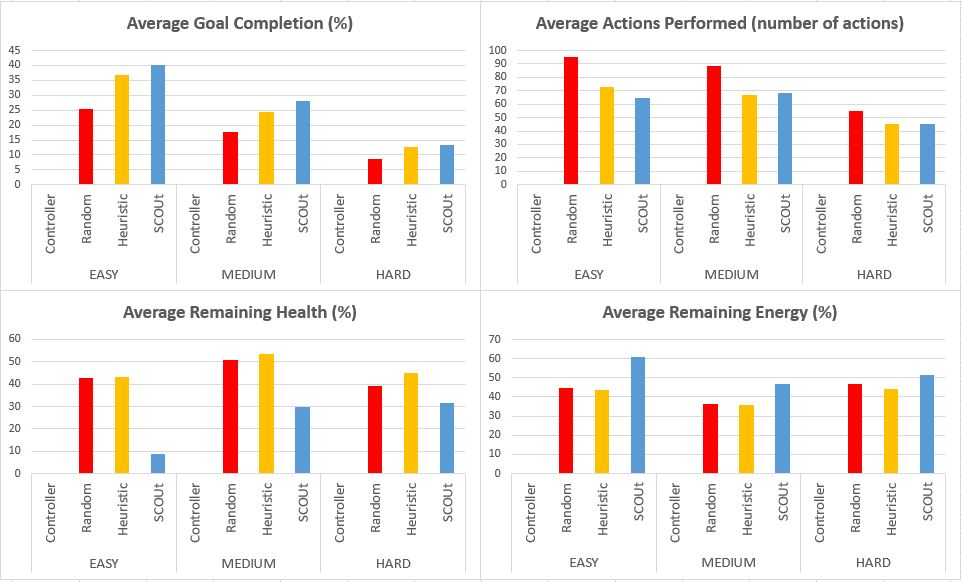
\includegraphics[width=1.0\columnwidth]{Figures/Results/Experiment1/MapWater.JPG}
  \caption[Experiment 1 Results: $SCOUt_{MW}$]{Performance results for $Random$, $Heuristic_{MW}$ and $SCOUt_{MW}$ attempting \textit{Map Water} in various environment difficulties.}
  \label{fig:mapwater_test_results}
\end{figure}


$SCOUt_{H}$ was tested in both \textit{Find Human} and \textit{Map Water}.
The results for each goal type are found in figures~\ref{fig:hybrid_findhuman_test_results} and~\ref{fig:hybrid_mapwater_test_results}, respectively.
Results for \textit{Find Human} operations show trends similar to the results for the $SCOUt_{FH}$ controller, except with smaller margins of increased performance against $Heuristic_{FH}$ and $Random$.
In environments of hard difficulty, $SCOUt_{H}$ shows performance levels that match with the heuristic controller.
This is likely caused by the fact that it was only trained on \textit{Find Human} for 15 iterations, along with a dilution effect caused by having a mixed memory set (from training on both goals).

\begin{figure}[H]
  \centering
  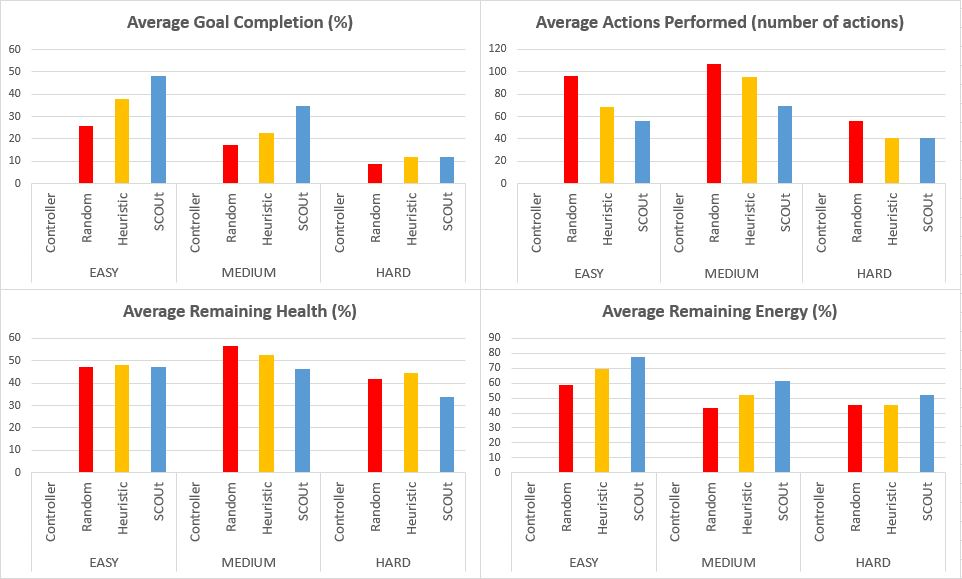
\includegraphics[width=1.0\columnwidth]{Figures/Results/Experiment1/HybridFindHuman.JPG}
  \caption[Experiment 1 Results: $SCOUt_{H}$ (Find Human)]{Performance results for $Random$, $Heuristic_{FH}$ and $SCOUt_{H}$ attempting \textit{Find Human} in various environment difficulties.}
  \label{fig:hybrid_findhuman_test_results}
\end{figure}

Results in \textit{Map Water} for the hybrid controller are nearly identical to the results seen in figure~\ref{fig:mapwater_test_results}.
The only notable difference is that average remaining health in easy environments was 21 percent instead of 9 percent.
Outside of this, performance scores and trends of all three controllers are roughly the same.
This suggests that operations based on mapping an element type are more difficult than would be expected.

\begin{figure}[H]
  \centering
  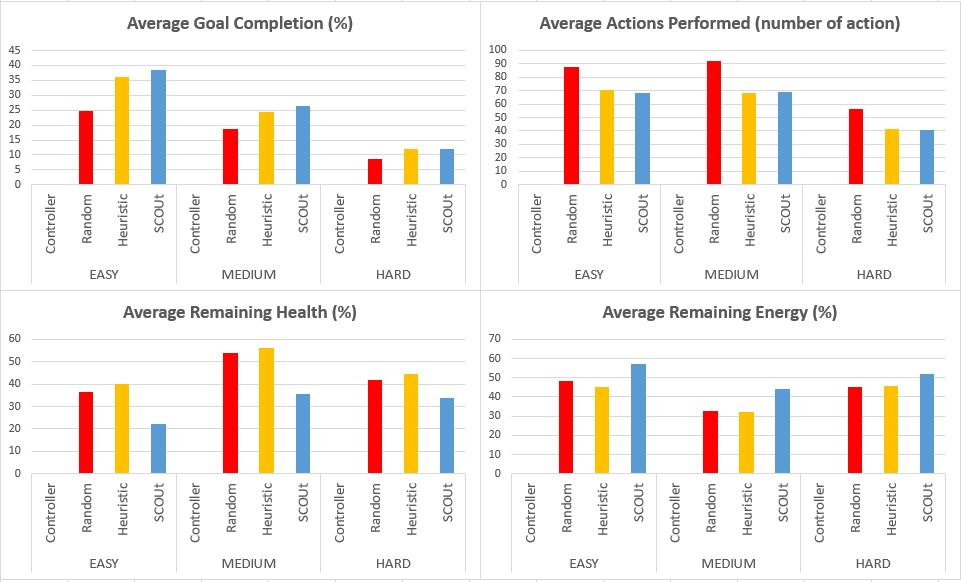
\includegraphics[width=1.0\columnwidth]{Figures/Results/Experiment1/HybridMapWater.JPG}
  \caption[Experiment 1 Results: $SCOUt_{H}$ (Map Water)]{Performance results for $Random$, $Heuristic_{MW}$ and $SCOUt_{H}$ attempting \textit{Map Water} in various environment difficulties.}
  \label{fig:hybrid_mapwater_test_results}
\end{figure}


\section{Experiment 2} \label{sec:experiment2}
The second experiment is broken into three tests: goal changing, sensor set changing, and additional training.
Goal changing, and sensor set changing are both designed to investigate the adaptability of each SCOUt controller.
Heuristic and random controllers are still used as baselines, but here the SCOUt controllers are also used as a baseline.
By comparing SCOUt controllers that were trained for the specific goal (in the case of goal changing) or un-altered (in the case of sensor set changing), performance changes can be studied on a SCOUt controller is applied in unexpected scenarios.
Following this, $SCOUt_{FH}$ and $SCOUt_{MW}$ are put through additional training on the goal they were not originally trained, to build two new controllers.
$SCOUt_{FH+}$ is the result of training on \textit{Map Water}, beginning with a copy of $SCOUt_{FH}$'s existing memory.
$SCOUt_{MW+}$ is the result of training on \textit{Find Human}, beginning with a copy of $SCOUt_{MW}$'s existing memory.
The new controllers will be tested to see how well SCOUt's control model is able to learn new tasks beginning with separate memory from another task.


\subsection{Goal Changing}
Goal changing tests the performance of $SCOUt_{FH}$ on the \textit{Map Water} goal, and the performance of $SCOUt_{MW}$ on the \textit{Find Human} goal.
The SCOUt controllers have no training on the new goal they are tested within, so behaviors are based purely on the controller's existing memory.
Every controller used in experimentation thus far is compared in these tests.
Tests are run in the same fashion (1000 operations per environment: 200 environments generated, each used 5 times), but in the results displayed, performance is averaged for each controller across all three environment difficulties.
This is done because it is already seen that each controller's performance scores show a relatively linear trend as difficulty increases (outside of the case with $SCOUt_{MW}$'s average remaining health).

Results for $SCOUt_{MW}$ in \textit{Find Human} operations are shown in figure~\ref{fig:goal_change_findhuman}.
Unsurprisingly, $SCOUt_{FH}$ takes the lead in every performance category, followed by $SCOUt_{H}$.
The primary interest here is $SCOUt_{MW}$'s ability to outperform $Heuristic_{FH}$.
Higher averages are seen in the number of actions performed and remaining energy, but this is likely due to the same hazard avoidance caveat discussed in Experiment 1 (section~\ref{sec:experiment1}).
This is also reflected in the fact that $SCOUt_{MW}$ has the lowest average remaining health out of all controllers, followed by $SCOUt_{H}$ (again, likely suffering from the same issue).
However, even though the average goal completion for $SCOUt_{MW}$ is less than $Heuristic_{FH}$, the margin of difference is only 1.5 percent.
This does lead to the idea that adaptability is present within SCOUt's control schema.
Using no prior training for how to find a human within an environment, the controller was still able to perform at the same level as a heuristic model.
Additionally, $SCOUt_{MW}$ also outperforms $Heuristic_{MW}$ in all categories excluding average remaining health.
This supports the primary focus of this paper, which is: demonstrating how autonomous control schemas built for one specific task are not inherently adaptable to new tasks, but there still exists underlying features of autonomous control that can be abstracted to create a unified control schema capable of achieving a variety of tasks.

\begin{figure}[H]
  \centering
  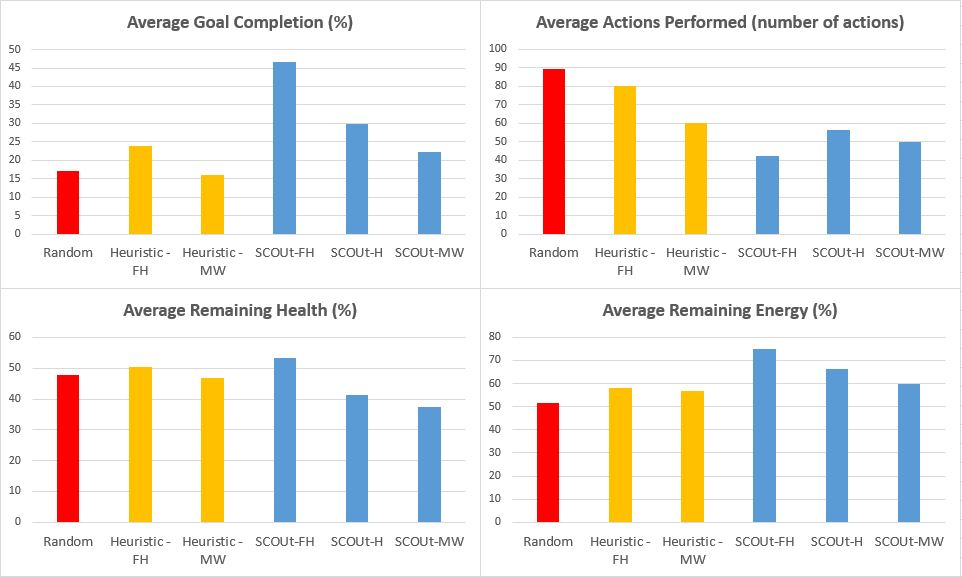
\includegraphics[width=1.0\columnwidth]{Figures/Results/Experiment2/GoalChange/FindHumanGoal.JPG}
  \caption[Experiment 2 - Goal Change Testing Results: $SCOUt_{MW}$]{Results for $SCOUt_{MW}$ in \textit{Find Human} operations compared against $Random$, $Heuristic_{FH}$, $Heuristic_{MW}$, $SCOUt_{FH}$, and $SCOUt_{H}$. While $SCOUt_{MW}$ did not have the best performance results out of all of the SCOUt controllers, it still performed better than $Random$ and both heuristic controllers in the majority of cases. This exemplifies the SCOUt control schema's ability to adapt to new goal types.}
  \label{fig:goal_change_findhuman}
\end{figure}

Goal change tests for the \textit{Map Water} goal (figure~\ref{fig:goal_change_mapwater}) hold some interesting results.
All three SCOUt controllers outperformed $Random$ and both heuristic controllers in every category except for average remaining health.
The fact that even $SCOUt_{FH}$ falls victim to poor performance in hazard avoidance suggests that there is level of inevitability for this control schema to eventually choose a detrimental action.
On the positive side, the goal completion rates for all three show superiority over the other controllers, with $SCOUt_{FH}$ taking the lead.
This could possibly be attributed to $SCOUt_{FH}$ having training where efficient sensor usage is highly rewarded.
Another interesting note is that $Heuristic_{FH}$ follows closely behind $Heuristic_{MW}$ in performance, and even takes the lead in average remaining health.
This speaks more toward the goal at hand than the control schema.
As stated previously in section~\ref{sec:experiment1}, element type mapping is likely a trickier task than expected.
The fact that the range of goal completion of heuristic and SCOUt controllers was ~24 - 28 percent supports this idea.

\begin{figure}[H]
  \centering
  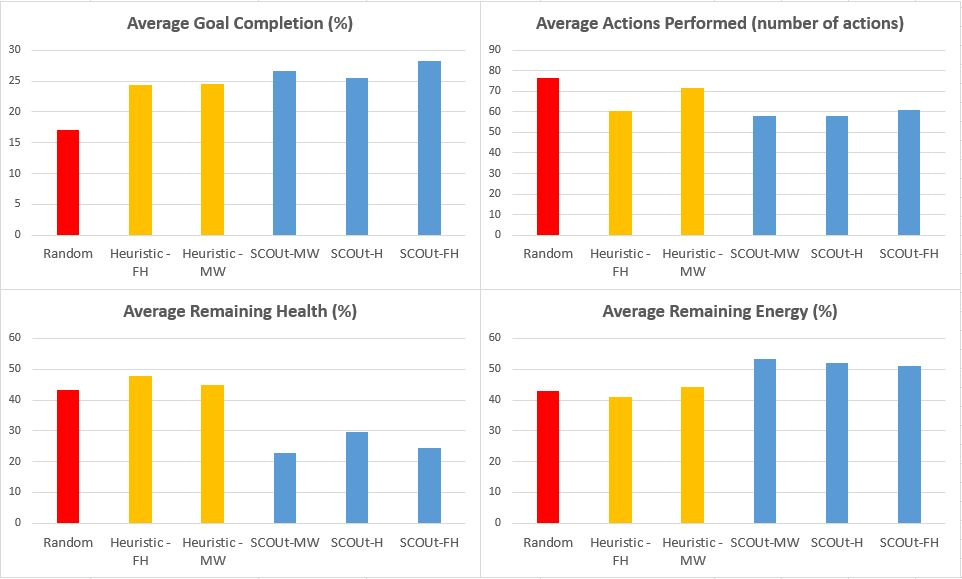
\includegraphics[width=1.0\columnwidth]{Figures/Results/Experiment2/GoalChange/MapWaterGoal.JPG}
  \caption[Experiment 2 - Goal Change Testing Results: $SCOUt_{FH}$]{Results for $SCOUt_{FH}$ in \textit{Map Water} operations compared against $Random$, $Heuristic_{FH}$, $Heuristic_{MW}$, $SCOUt_{MW}$, and $SCOUt_{H}$. Results show that all SCOUt controllers performed at roughly the same level in all categories. In all categories besides average remaining health, the SCOUt controllers perform best. $SCOUt_{FH}$ takes the lead in goal completion out of all controllers. This again supports the adaptability of the SCOUt control schema.}
  \label{fig:goal_change_mapwater}
\end{figure}


\subsection{Sensor Set Changing} \label{sec:sensor_change}
Sensor set changing analyzes how a SCOUt controller is able to perform the goal they were trained for after removing a sensor that it had learned to use for achieving the given task.
Tests are conducted in the same manner as the goal change tests, where 1000 tests per environment difficulty are run, and performance results are averaged across each difficulty level.
The controllers used in each test are $Random$, the heuristic controller designed for the given goal, the original SCOUt controller trained on the goal (denoted as $<controller-name> - All$), and copies of the same SCOUt controller setup with a variation of available sensors.

First, the results for the \textit{Map Water} goal (figure~\ref{fig:change_sensors_mapwater}) are examined.
Because only water and elevation sensors are used in \textit{Map Water} operations (and elimination of the water sensor would result in the inability to achieve any level of goal completion), only one agent variation is considered ($SCOUt_{MW} - No Elevation$).
We see $SCOUt_{MW} - All$ and $SCOUt_{MW} - No Elevation$ topping each performance category besides average remaining health.

\noindent
$SCOUt_{MW} - No Elevation$ outperforms $SCOUt_{MW} - All$ in each category outside of remaining health.
This is likely due to the fact that $SCOUt_{MW} - No Elevation$ only has a water sensor, and therefore can only choose to scan for water, or move.
The drop in average remaining health could then be attributed to the controller's lack of ability to detect hazardous drops in elevation.
If this is true, it would suggest that SCOUt's ability to learn hazard avoidance is not entirely flawed.

\begin{figure}[H]
  \centering
  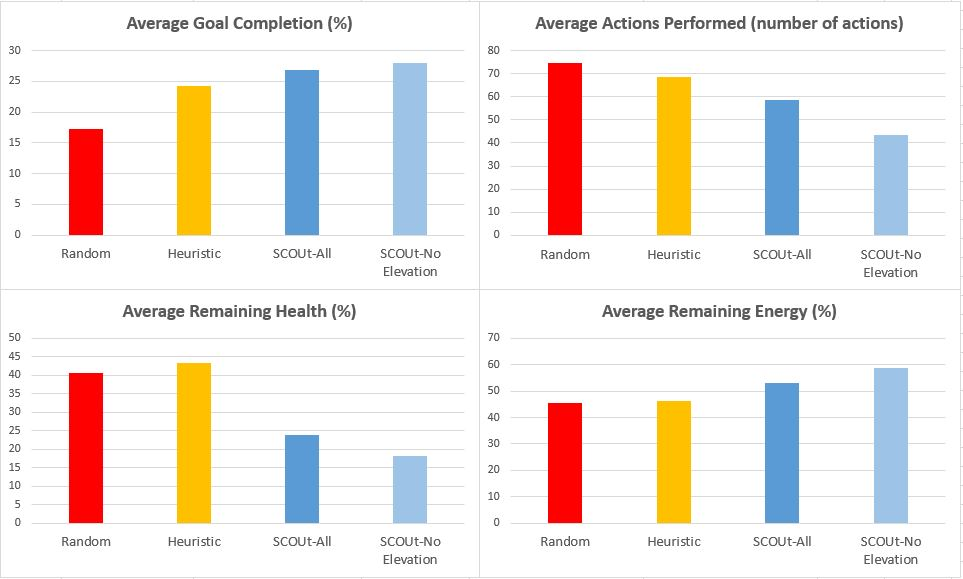
\includegraphics[width=1.0\columnwidth]{Figures/Results/Experiment2/SensorChange/MapWater.JPG}
  \caption[Experiment 2 - Sensor Set Changing Results: $SCOUt_{MW}$]{Performance results for $SCOUt_{MW}$ when its elevation sensor was removed ($SCOUt_{MW} - No Elevation$) in \textit{Map Water} operations. It was also compared against an un-altered version of $SCOUt_{MW}$ ($SCOUt_{MW} - All$), $Heuristic_{MW}$, and $Random$. The results show that the SCOUt control schema was able to perform adaptively without the availability of the elevation sensor.}
  \label{fig:change_sensors_mapwater}
\end{figure}

Moving on to testing with the $SCOUt_{FH}$, we see positive results in figure~\ref{fig:change_sensors_findhuman}.
Four variations of sensor sets are examined by removing the elevation, water, temperature and then decibel sensors.
The four respective controllers are denoted as $SCOUt_{FH} - No Elevation$, $SCOUt_{FH} - No Water$, $SCOUt_{FH} - No Temp$ and $SCOUt_{FH} - No Decibel$.
In three out of the four performance categories, the majority of SCOUt controllers perform best.
The only SCOUt controller with a large performance difference among the five is $SCOUt_{FH} - No Decibel$.
Surveillance of decibel values within the environment is a critical behavior to tracking down the location of the human anomaly.
The fact that $SCOUt_{FH} - No Decibel$ shows performance drops demonstrates the ability of SCOUt's control schema to learn pattern recognition behaviors for goal completion.
Despite the handicap of having no decibel sensor, the controller still outperformed $Random$ and $Heuristic_{FH}$ in goal completion, number of actions performed, and remaining energy.
This further demonstrates the adaptability of the SCOUt control schema.
$SCOUt_{FH} - No Decibel$ likely was still able to pick up on the agent using its temperature sensor, which would require the agent to be moved into closer proximity to the human to detect their heat signature.
Removal of each other sensor surprisingly had little to no effect on performance compared to $SCOUt_{FH} - All$.
Performance in all categories aside from remaining health for all of these controllers were roughly double $Heuristic_{FH}$'s and triple $Random$'s.
These results reveal a strong level of adaptability within SCOUt's memory-based reinforcement learning schema when dealing with new agent setups.

\begin{figure}[H]
  \centering
  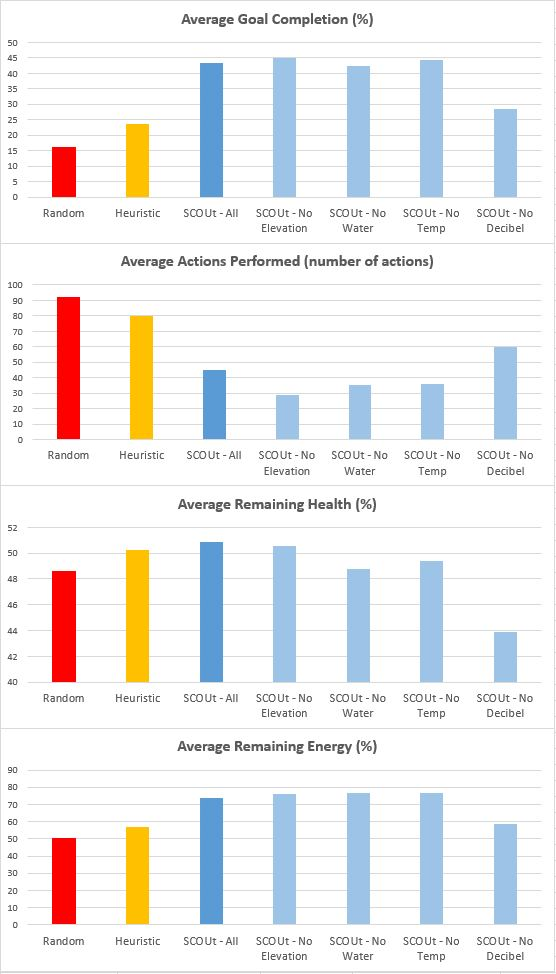
\includegraphics[width=0.65\columnwidth]{Figures/Results/Experiment2/SensorChange/FindHuman.JPG}
  \caption[Experiment 2 - Sensor Set Changing Results: $SCOUt_{FH}$]{Performance results for several variations of SCOUt controllers with a sensor removed in \textit{Find Human} operations. These variations were tested against the un-altered SCOUt controller ($SCOUt_{FH}$), $Heuristic_{FH}$, and $Random$. Results show that SCOUt's control schema was able to adapt to each situation where a sensor was removed. The SCOUt controllers outperform $Heuristic_{FH}$ and $Random$ in the majority of performance categories. The only noticeable decline in SCOUt's performance is with the removal of the decibel sensor ($SCOUt_{FH} - No Decibel$). This is likely due to decibel readings being a key indicator of a human's location.}
  \label{fig:change_sensors_findhuman}
\end{figure}


\subsection{Additional Training}
The final task of Experiment 2 was to observe how quickly a controller is able to improve and learn new behaviors related to a different goal.
Two new controllers are retrained and then tested for completing a new goal.
$SCOUt_{FH+}$ begins with a copy of $SCOUt_{FH}$'s trained memory and is then retrained for completing \textit{Map Water}.
$SCOUt_{MW+}$ begins with a copy of $SCOUt_{MW}$'s trained memory and is then retrained for completing \textit{Find Human}.
The retraining for each new controller follows the same setup seen in section~\ref{sec:training}.
Once completed, each controller will be tested in the new goal they were trained against $SCOUt_{FH}$, $SCOUt_{MW}$, the goal's respective heuristic controller, and the $Random$ controller.
It is expected that the retrained controllers will perform better than the original SCOUt controller whose memory they use.
Additionally, we would like to see measures of performance that are better than the heuristic controller and near the levels of the original SCOUt controller that was trained for the given goal.
Tests are conducted in the same fashion as seen in Change Goal and Change Water testing.
One thousand operations are conducted per environment difficulty and the results are averaged from the total 3000 operations.

Retraining for both new controllers show trends that are similar to all training seen in the original controllers.
$SCOUt_{FH+}$ retraining on \textit{Map Water} (figure~\ref{fig:findhumanplus_training_results}) does not show any increase in goal completion and a decline in the average health is seen.
Remaining energy and number of actions performed climb and fall for the same reason discussed with the original

\noindent
$SCOUt_{MW}$ controller, where short operations caused by health depletion reflect in less overall activity.
$SCOUt_{MW+}$ shows major improvement in goal completion while maintaining a low average number of actions taken (as seen in figure~\ref{fig:mapwaterplus_training_results}).
Additionally, minor climbs in the average remaining health and energy of the agent suggest that the controllers learn to operate more efficiently.


\begin{figure}[H]
  \centering
  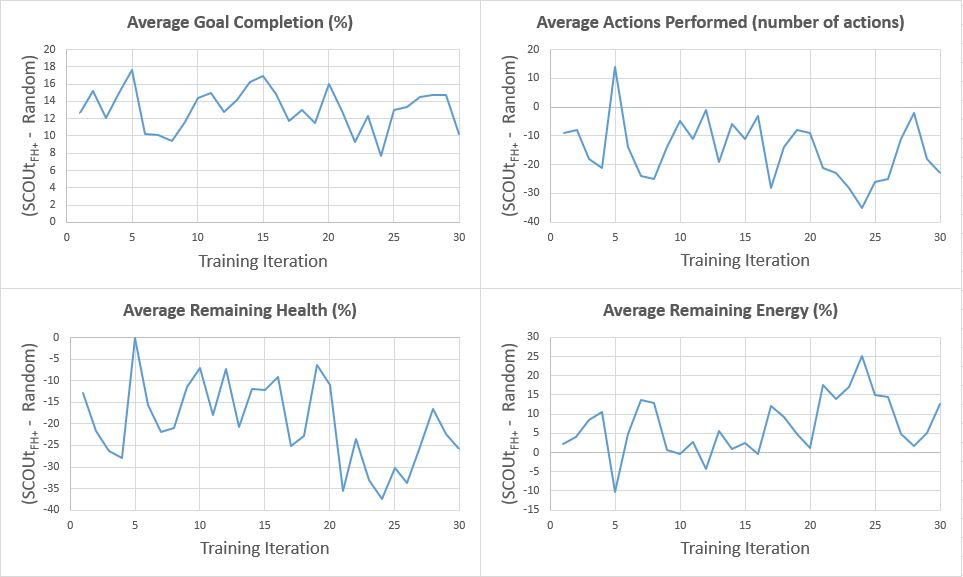
\includegraphics[width=0.9\columnwidth]{Figures/Results/Experiment2/AdditionalTraining/FHPlus_Training.JPG}
  \caption[Experiment 2 - Additional Training Results: $SCOUt_{FH+}$]{Iteration testing performance results for $SCOUt_{FH+}$ attempting \textit{Map Water}. All graphs show the controller's average difference in performance compared to $Random$ ($SCOUt_{FH+}$ average - $Random$ average) VS the number of training iterations completed.}
  \label{fig:findhumanplus_training_results}
\end{figure}

\begin{figure}[H]
  \centering
  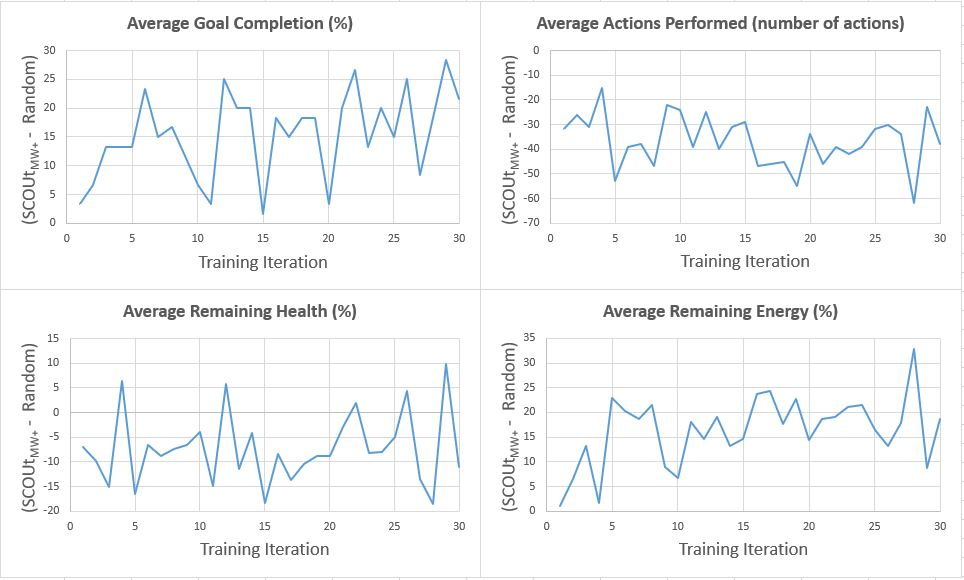
\includegraphics[width=0.9\columnwidth]{Figures/Results/Experiment2/AdditionalTraining/MWPlus_Training.JPG}
  \caption[Experiment 2 - Additional Training Results: $SCOUt_{MW+}$]{Iteration testing performance results for $SCOUt_{MW+}$ attempting \textit{Map Water}. All graphs show the controller's average difference in performance compared to $Random$ ($SCOUt_{MW+}$ average - $Random$ average) VS the number of training iterations completed.}
  \label{fig:mapwaterplus_training_results}
\end{figure}


After training, $SCOUt_{FH+}$ was tested for performance in \textit{Map Water} operations against the original $SCOUt_{FH}$, $SCOUt_{MW}$, $Heuristic_{MW}$, and $Random$.
The results seen in figure~\ref{fig:findhumanplus_test_results} show minor improvements over $SCOUt_{FH}$ for goal completion.
Remaining health is slightly lower, but the number actions taken and remaining energy where still equivalent to that of

\noindent
$SCOUt_{FH}$.
Again, another SCOUt controller is outranking the $Heuristic_{MW}$ controller designed specifically for the goal at hand in all categories except remaining health.
While hazard avoidance is still an issue, it can still be argued that this controller is operating efficiently as it shows better performance averages in all other categories.

\begin{figure}[H]
  \centering
  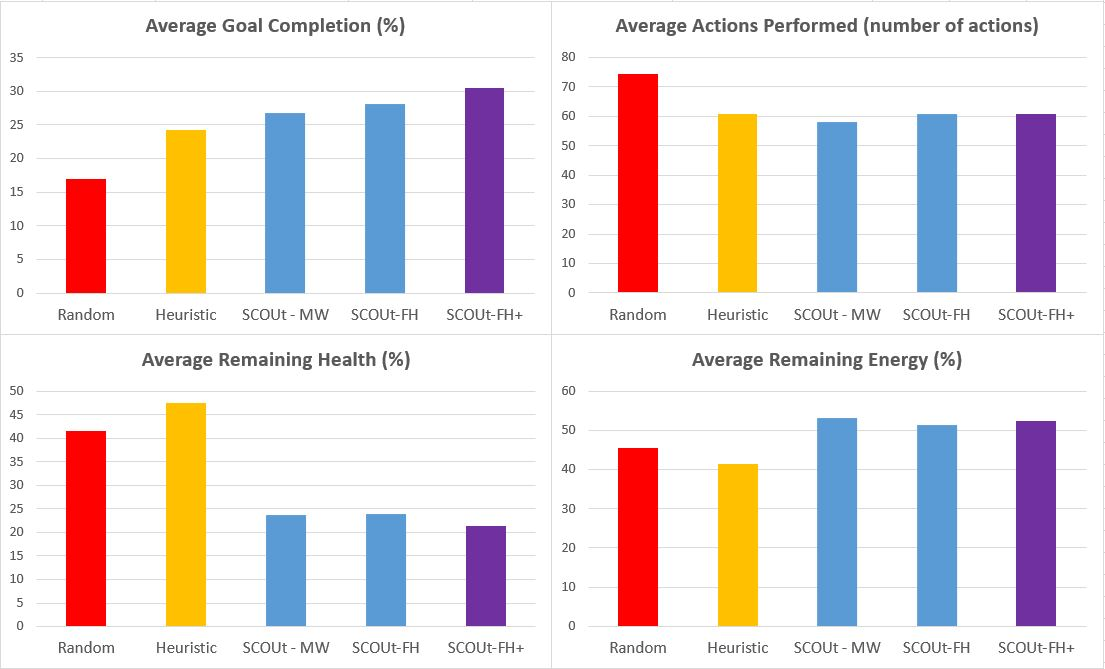
\includegraphics[width=1.0\columnwidth]{Figures/Results/Experiment2/AdditionalTraining/FindHumanPlus.JPG}
  \caption[Experiment 2 - Additional Training Testing Results: $SCOUt_{FH+}$]{Iteration testing performance results for $SCOUt_{FH+}$ attempting \textit{Map Water}. All graphs show the controller's average difference in performance compared to $Random$ ($SCOUt_{FH+}$ average - $Random$ average) VS the number of training iterations completed.}
  \label{fig:findhumanplus_test_results}
\end{figure}


Figure~\ref{fig:mapwaterplus_test_results} shows the performance of $SCOUt_{MW+}$ against the original $SCOUt_{MW}$,

\noindent
$SCOUt_{FH}$, $Heuristic_{FH}$, and $Random$ in \textit{Find Human} operations.
Here we see that

\noindent
$SCOUt_{MW+}$ does outrank $SCOUt_{MW}$ and the heuristic controller as expected.
$SCOUt_{FH}$ still takes the lead in every category, but the new controller does show major overall improvements due to its additional training.
This further supports the argument that a memory-based reinforcement learning model holds many adaptive attributes for facing new situations.


\begin{figure}[H]
  \centering
  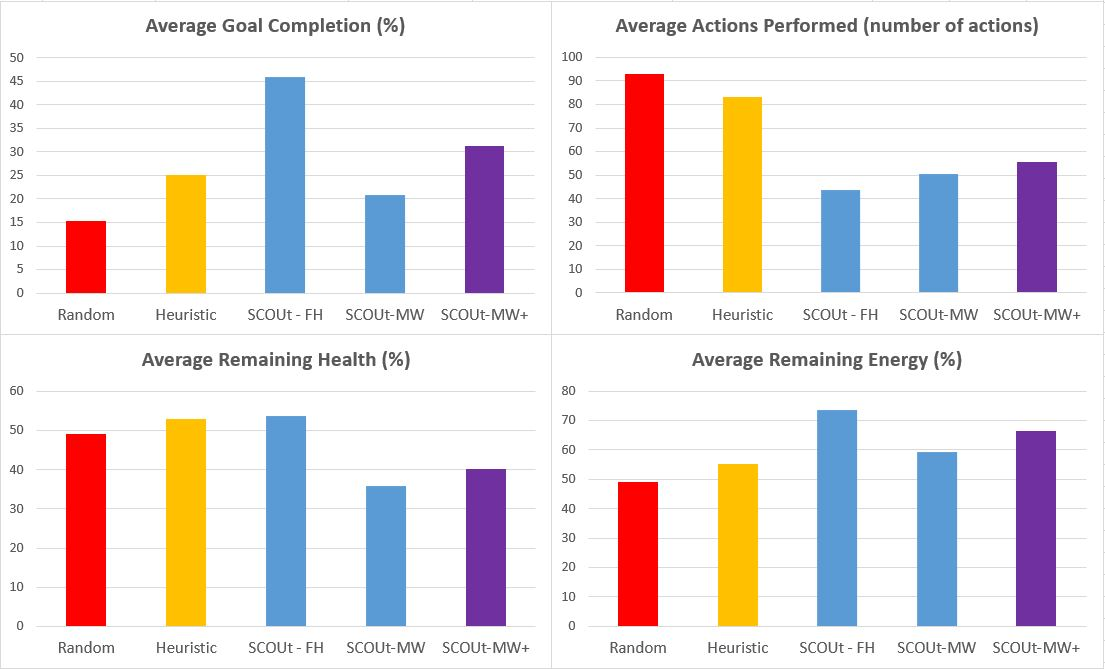
\includegraphics[width=1.0\columnwidth]{Figures/Results/Experiment2/AdditionalTraining/MapWaterPlus.JPG}
  \caption[Experiment 2 - Additional Training Testing Results: $SCOUt_{MW+}$]{Iteration testing performance results for $SCOUt_{MW+}$ attempting \textit{Map Water}. All graphs show the controller's average difference in performance compared to $Random$ ($SCOUt_{MW+}$ average - $Random$ average) VS the number of training iterations completed.}
  \label{fig:mapwaterplus_test_results}
\end{figure}



\section{Discussion}
Testing revealed that SCOUt's control schema was in fact adaptive to new tasks.
In Experiment 2, we see SCOUt controllers performing better than random and heuristic approaches, even when faced with disadvantages, such as lack of sensors or no knowledge of how to complete a goal.
These are features that are not seen in the heuristic models.
The heuristic approaches were able to perform adequately in their respective goals, but due to the goal-specific logic that was used in their control models, they did not perform well when presented to a new goal type.
There is an issue with SCOUt's hazard avoidance, as results in all testing showed poor ranking in the category of average remaining health.
Despite this, SCOUt still showed superior results in the other three categories for the majority of tests.
It is suspected that if the hazard avoidance issue were to be fixed, this control model would achieve even better results in all performance categories.
Another notable feature within the results was $SCOUt_{FH}$'s performance in the goal change testing (figure~\ref{fig:goal_change_findhuman}).
Here we saw that the SCOUt controller without a decibel sensor equipped showed noticeable performance drops, but still performed better than the random and heuristic controllers.
This signifies two things.
First, SCOUt is learning behaviors related to goal completion.
Changes in decibel levels within the environment are the strongest indicator to finding a human's location.
The fact that $SCOUt_{FH} - No Decibel$ showed lower performance compared to all other SCOUt controllers in the test suggests that the controller has learned search behaviors related to analyzing the environment.
Second, because SCOUt was still able to outperform the random and heuristic controllers despite its disadvantage in this situation, I argue that SCOUt's control model is in fact adaptive.
While $SCOUt_{FH} - No Decibel$ would not be able to pick up on the human's sound effect, it was able to use other learned information to still guide it to successfully goal completions.
